\documentclass [a4paper] {article}

\usepackage[spanish]{babel} 
\usepackage[utf8]{inputenc} 
\usepackage{multirow} 
\usepackage{float} 

\title{R-PL5}
\author{Gabriel López, Sergio Sanz, Álvaro Zamorano}

\usepackage{Sweave}
\begin{document}
\Sconcordance{concordance:G16-p5.tex:G16-p5.Rnw:%
1 10 1 1 0 30 1 1 2 1 0 1 1 3 0 1 2 5 1 1 2 1 0 1 1 3 0 1 2 5 1 1 2 1 0 %
1 1 22 0 1 2 2 1 1 2 7 0 1 2 30 1 1 3 2 0 1 1 3 0 1 2 5 1 1 2 7 0 1 1 7 %
0 1 2 1 1 1 2 8 0 1 2 2 1 1 2 1 0 1 1 17 0 1 2 2 1 1 2 7 0 1 2 4 1 1 2 %
1 0 1 1 3 0 1 2 9 1 1 2 7 0 1 2 1 1 1 2 1 0 1 1 6 0 1 2 1 1 1 2 7 0 1 2 %
2 1 1 2 1 0 1 1 17 0 1 2 2 1 1 2 7 0 1 2 10 1 1 2 12 0 1 2 1 1 1 2 1 0 %
1 1 6 0 1 2 2 1 1 2 7 0 1 2 2 1 1 2 1 0 1 1 18 0 1 2 2 1 1 2 7 0 1 2 13 %
1 1 2 1 0 3 1 3 0 1 2 4 1 1 2 1 0 2 1 3 0 1 2 15 1 1 2 1 0 1 1 6 0 1 2 %
3 1 1 2 1 0 1 1 3 0 1 2 3 1 1 2 1 0 2 1 3 0 1 2 11 1 1 2 7 0 1 2 3 1 1 %
2 1 0 1 1 3 0 1 2 3 1 1 2 1 0 2 1 3 0 1 2 10 1 1 2 11 0 1 2 8 1 1 2 1 0 %
1 1 1 2 1 0 3 1 6 0 1 2 3 1 1 2 7 0 1 2 1 1}


\maketitle

\graphicspath{ {./tmp/} }

\section{Ejercicio realizado en clase.}

\subsection{K-vecinos}
\bigskip
A partir del siguiente conjunto de calificaciones académicas,formados por dos notas: teoría y laboratorio, 
que tendrán valores entre 0 y 5, realizar un análisis de detección de datos anómalos utilizando el algoritmo
\textbf{K-vecinos}.

\begin{table}[H]
\begin{center}
\begin{tabular}{|c|c|c|c|c|}
\hline
Alumno & Teoría & Laboratorio\\
\hline \hline
A1 & 4 & 4 \\ \hline
A2 & 4 & 3 \\ \hline
A3 & 5 & 5 \\ \hline
A4 & 1 & 1 \\ \hline
A5 & 5 & 4 \\ \hline
\end{tabular}
\end{center}
\end{table}

En primer lugar se introducirán los datos en forma de matriz y se hará la traspuesta de esta.
\begin{Schunk}
\begin{Sinput}
> muestra = matrix(c(4,4,4,3,5,5,1,1,5,4),2,5)
> muestra = t(muestra)
\end{Sinput}
\end{Schunk}

\bigskip
En segundo lugar, calculamos las distancias euclídeas entre todos los puntos y los almacenamos 
en una matriz. El cálculo de las distancias lo realizamos mediante la función \textbf{as.matrix}. 

\bigskip
\begin{Schunk}
\begin{Sinput}
> distancias = as.matrix(dist(muestra))
> distancias = matrix(distancias,5,5)
\end{Sinput}
\end{Schunk}

\bigskip
En tercer lugar, ordenamos las columnas de la matriz de distancias por los valores de cada una de
las filas de menor a mayor. Se tiene en cuenta el \textbf{tercer} vecino, por lo que debemos estudiar la cuarta 
fila de la matriz ya que se tiene en cuenta la distancia de un punto consigo mismo. Se obtienen las 
muestras cuyo suceso es anómalo o outlier, el grado de outlier es \texttt{2.5.}
\begin{Schunk}
\begin{Sinput}
> source("./Funciones/anomalosKVecinos.R")
> anomalosKVecinos
\end{Sinput}
\begin{Soutput}
function (distancias, muestra, k, grado,dimensiones) {
    tmp<-""

    for(i in 1:(length(muestra)/dimensiones)){
        distancias[,i] = sort(distancias[,i])
        if(distancias[k+1,i] > grado) {
            valor<-""
            for (j in 1:dimensiones){
                valor<-paste(valor,muestra[k+1,j])
            }
            tmp<-paste(tmp,"La muestra ", i, 
                " con valor (", valor, ") es outlier - ",sep="")
        }
    }

    return(tmp)
}
\end{Soutput}
\end{Schunk}

\bigskip
Procedemos a su ejecución:
\begin{Schunk}
\begin{Sinput}
> (anomalosKVecinos(distancias,muestra,3,2.5,2))
\end{Sinput}
\begin{Soutput}
[1] "La muestra 4 con valor ( 1 1) es outlier - "
\end{Soutput}
\end{Schunk}

\bigskip
Es importante indicar que la función necesita conocer el número de \textbf{dimensiones} que tiene
la muestra.

\subsection{Caja y bigotes.}
\bigskip
A partir del siguiente conjunto de valores de resistencia y densidad para diferentes tipos de hormigón,
se hará un análisis para la detección de outliers utilizando medidas de ordenación sobre la resistencia
con el método de \textbf{Caja y Bigotes}.

\begin{table}[H]
\begin{center}
\begin{tabular}{|c|c|c|c|c|}
\hline
Hormigón & Resistencia & Densidad\\
\hline \hline
H1 & 3 & 2 \\ \hline
H2 & 3.5 & 12 \\ \hline
H3 & 4.7 & 4.1 \\ \hline
H4 & 5.2 & 4.9 \\ \hline
H5 & 7.1 & 6.1 \\ \hline
H6 & 6.2 & 5.2 \\ \hline
H7 & 14 & 5.3 \\ \hline
\end{tabular}
\end{center}
\end{table}

\bigskip
En primer lugar, introducimos los datos en una matriz y lo convertimos a dataframe para que el trabajo con las 
columnas sea más cómodo.
\begin{Schunk}
\begin{Sinput}
> muestra = t(matrix(c(3,2,3.5,12,4.7,4.1,5.2,4.9,7.1,6.1,6.2,5.2,14,5.3),
+         2,7,dimnames = list(c("r","d"))))
> muestra = data.frame(muestra)
\end{Sinput}
\end{Schunk}

\bigskip
En segundo lugar:
\begin{enumerate}
\item Se determina el grado de outlier de forma arbitraria. El valor dado es \texttt{1.5}.
\item Se ordenan los datos y se obtienen los cuartiles.
\begin{Schunk}
\begin{Sinput}
> cuar1 <- quantile(muestra$r,0.25)
> cuar3 <- quantile(muestra$r,0.75)
\end{Sinput}
\end{Schunk}

\item Se calculan los límites del intervalo.
\begin{Schunk}
\begin{Sinput}
> int = c(cuar1 - 1.5 * (cuar3 - cuar1),cuar3 + 1.5*(cuar3-cuar1))
\end{Sinput}
\end{Schunk}

\item Se identifican como outliers los valores que quedan fuera del intervalo.
\begin{Schunk}
\begin{Sinput}
> for(i in 1:length(muestra$r)){
+      if(muestra$r[i] < int[1] || muestra$r[i] > int[2]){
+            print("El suceso "); print(i);print(" con valor ");
+            print(muestra$r[i]); print(" es un suceso anomalo o outlier")
+       }
+ }
\end{Sinput}
\begin{Soutput}
[1] "El suceso "
[1] 7
[1] " con valor "
[1] 14
[1] " es un suceso anomalo o outlier"
\end{Soutput}
\end{Schunk}
\end{enumerate}

\bigskip
Por último, mostramos el diagrama de caja y bigotes donde se identifica el valor anómalo.
\begin{Schunk}
\begin{Sinput}
> source("./Funciones/Bigotes.R")
> bigotes(muestra$r,"bigotes.png",1.5)
\end{Sinput}
\end{Schunk}
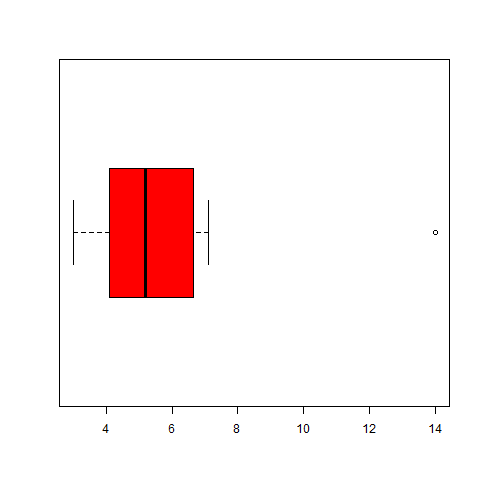
\includegraphics[width=\textwidth]{bigotes}

\subsection{Desviación Típica.}
\bigskip
Ahora con los mismos datos del apartado anterior deseamos realizar un análisis de detección de datos 
anómalos utilizando medidas de dispersión sobre la densidad con el método de \textbf{Desviación Típica}.
\begin{enumerate}
\item Se determina el grado de outlier de forma arbitraria. El valor dado es \texttt{2}.
\item Se obtiene la media aritmética.
\begin{Schunk}
\begin{Sinput}
> media<-mean(muestra$d)
\end{Sinput}
\end{Schunk}
\item Se obtiene la desviación típica.
\begin{Schunk}
\begin{Sinput}
> sdd<-sd(muestra$d)
> desviacion<-sqrt((sdd^2)*((length(muestra$d)-1)/length(muestra$d)))
\end{Sinput}
\end{Schunk}
\item Y por último, se calculan los límites del intervalo para los valores atípicos.
\begin{Schunk}
\begin{Sinput}
> intdes<-c(media-2*desviacion,media+2*desviacion)
\end{Sinput}
\end{Schunk}
\item Se identifican como outliers los valores que quedan fuera del intervalo.
\begin{Schunk}
\begin{Sinput}
> for(i in 1:length(muestra$d)){
+      if(muestra$d[i] < intdes[1] || muestra$d[i] > intdes[2]){
+            print("El suceso "); print(i);print(" con valor ");
+            print(muestra$d[i]); print(" es un suceso anomalo o outlier")
+       }
+ }
\end{Sinput}
\begin{Soutput}
[1] "El suceso "
[1] 2
[1] " con valor "
[1] 12
[1] " es un suceso anomalo o outlier"
\end{Soutput}
\end{Schunk}
\end{enumerate}

\end{document}
